\item El estado que ha realizado la menor cantidad de órdenes. Se debe mostrar también el total de ordenes que haya entregado.

\begin{lstlisting}
ordenes = π state,orderid (customer ⨝ orders)

por_estado = γ state; count(orderid)→total (ordenes)

minimo = γ ; min(total)→menor (por_estado)

resultado = π state,total (σ total = menor (por_estado ⨯ minimo))

resultado
\end{lstlisting}

\begin{center}
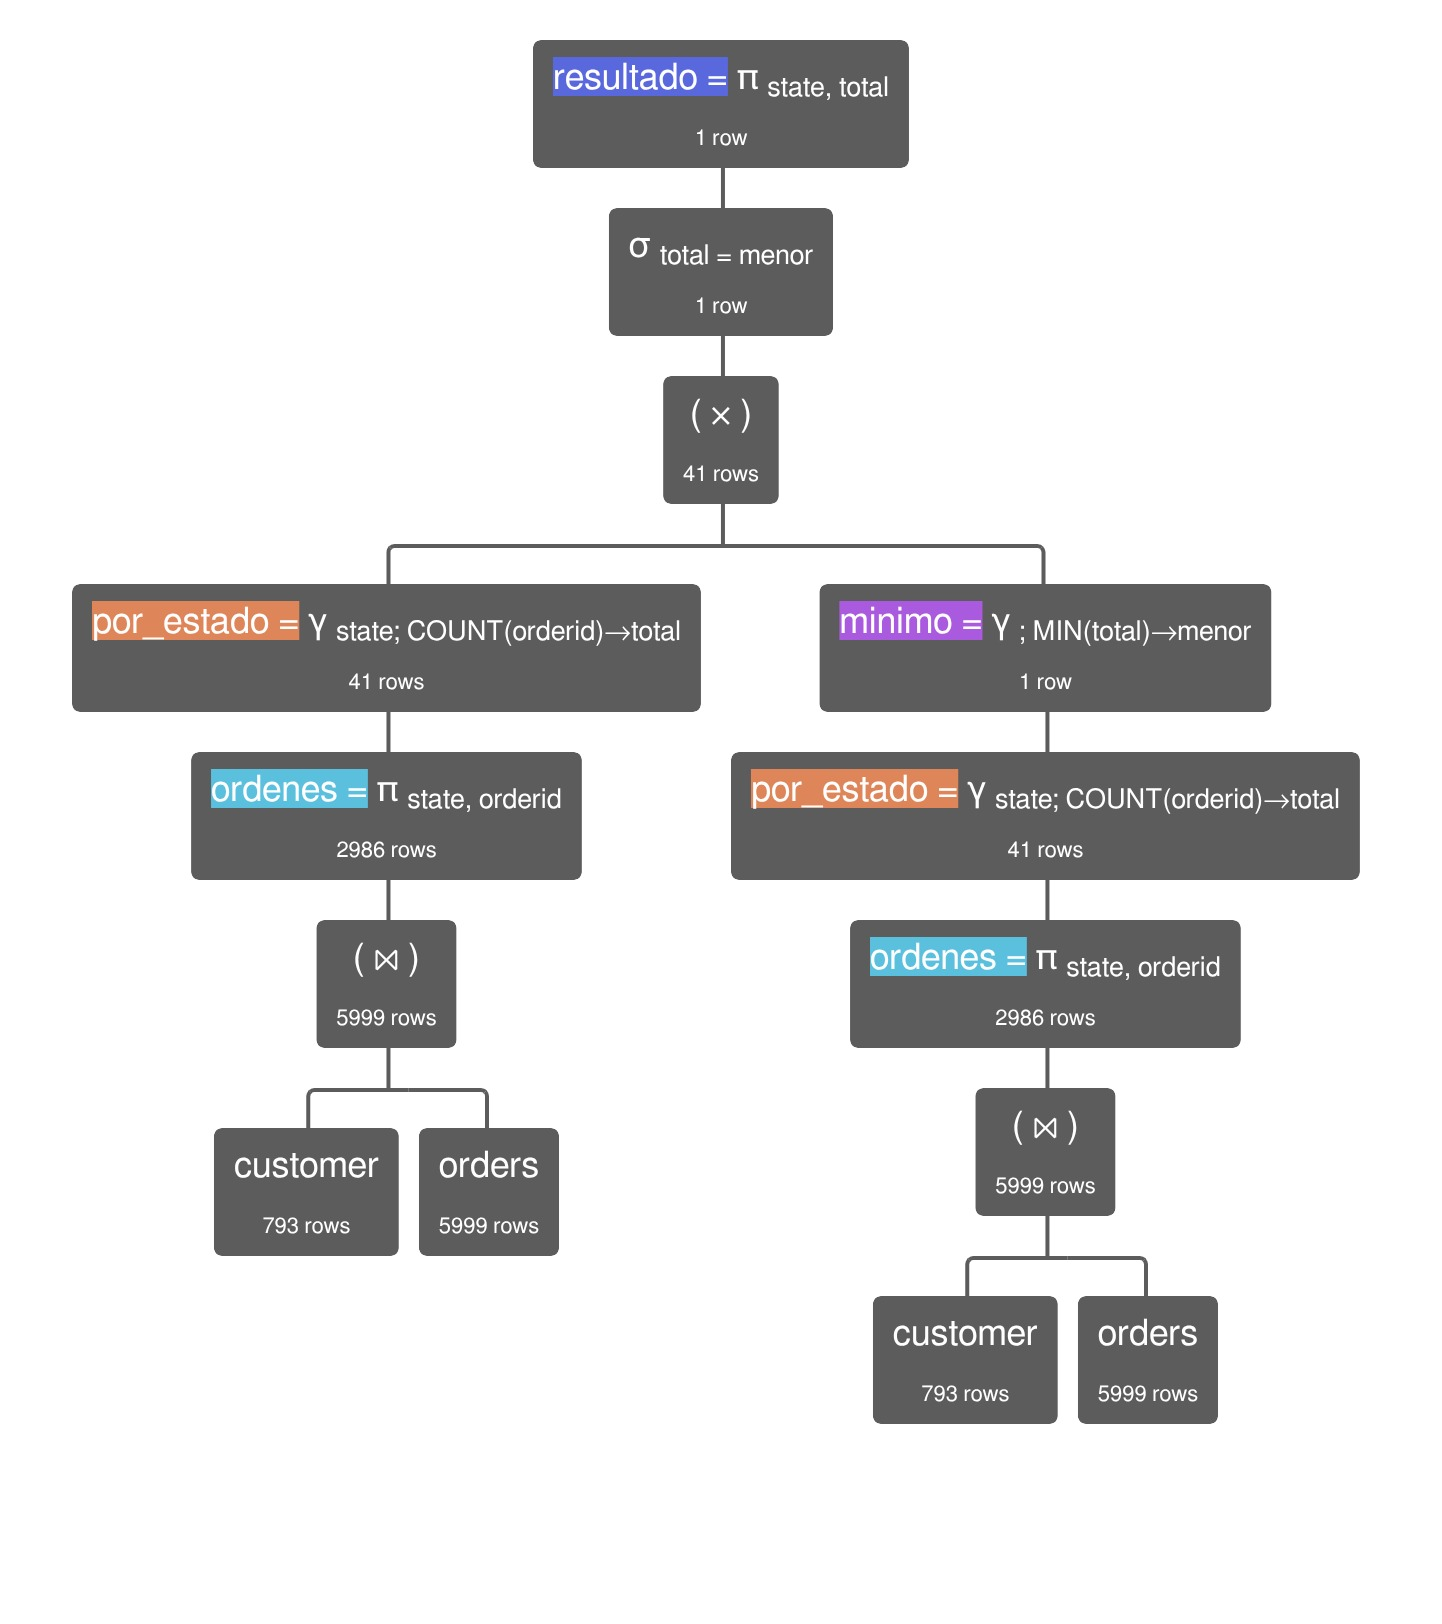
\includegraphics[width=0.65\textwidth]{figuras/2i_1.jpg}
\end{center}

\begin{center}
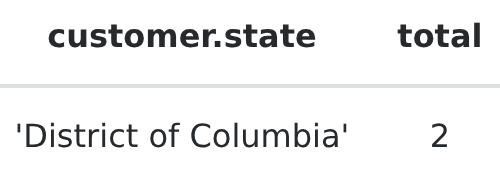
\includegraphics[width=0.4\textwidth]{figuras/2i_2.png}
\end{center}

\newpage
